
%\begin{center}
%\Large\textbf{Short-Baseline Neutrino Program}
%\end{center}

The discovery that neutrinos undergo oscillation in their flavor, and thus are massive particles, serves as one of the first pieces of evidence for physics beyond the Standard Model (SM) of particle physics. The prevailing description of neutrino oscillations provided by the Pontecorvo-Maki-Nakagawa-Sakata (PMNS) matrix characterizes the flavor change as a result that the neutrino flavor eigenstates ($\nu_{e}, \nu_{\mu}, \nu_{\tau}$) are a linear combination of the neutrino mass eigenstates ($\nu_{1}, \nu_{2}, \nu_{3}$). The rotation from the mass eigenstates to the flavor eigenstates is governed by three angles $\theta_{i,j}$, where $i$ and $j$ correspond to the mass eigenstates with $i < j$, and a phase $\delta$ which determines magnitude of charge-parity (CP) violation within the neutrino sector. Additionally, the flavor change of the neutrinos depends on the ratio neutrino energy and the distance traveled by the neutrino (often referred to as the baseline) as well as the difference in the square of the mass eigenstates $\Delta m_{ji}^{2}$. Neutrinos produced in the atmosphere \cite{No1, No2, No3}, in nuclear reactors \cite{No4, No5, No6}, in the sun \cite{No7, No8, No9}, as well as in man-made particle accelerators \cite{No10, No11, No12} have been used to study the phenomenon of neutrino oscillations. The exact ordering of the neutrino mass states, known as the mass hierarchy, as well as the size of the CP-violating phase $\delta$ are, as yet, unknown. These quantities remain one of the last major pieces of the Standard Model of particle physics and offer the opportunity to answer such fundamental questions as:

\begin{itemize}
\item[1)] \textbf{What is the origin of the matter/antimatter asymmetry in the universe?}

\item[2)] \textbf{Do we understand the fundamental symmetries of the universe?}

\item[3)] \textbf{Is the three-flavor paradigm of the Standard Model for neutrino oscillation the accurate description for neutrino interactions?}
\end{itemize}

Into this experimental landscape, there exists a set of series of experimental measurements which suggest that the three-flavor paradigm of neutrino oscillations is incomplete. Two general classes of anomalous observations may point to additional physics beyond the SM  in the neutrino sector.

\begin{itemize}
\item \textbf{The disappearance signal in low energy electron anti-neutrinos from reactor neutrino experiments \cite{No13} \textit{(``Reactor Neutrino Anomaly'')} and Mega-Curie radioactive electron neutrino sources in Gallium \cite{No14, No15} \textit{(``Gallium Anomaly'')}}

\item \textbf{The electron-like excess from muon neutrino (and anti-neutrino) particle accelerators \textit{(``LSND/MiniBooNE Anomaly'')} \cite{No16, No17}}

\end{itemize}

Neither of these anomalies can be accounted for by the standard three-flavor oscillations of the SM and may hint at the existence of additional neutrino states with larger mass difference ($\Delta m_{new}^{2}\geq 0.1 eV^{2}$) which participate in the mixing of the flavour states (referred to as ``sterile neutrinos''). Definitive evidence of the existence of new neutrino states would be a revolutionary discovery with broad implications for both particle physics and cosmology. Moreover, in order for future accelerator based neutrino experiments to disentangle the mass hierarchy and search for CP-violation, the oscillation framework must be concretely known and precisely measured.

Liquid Argon Time Projection Chambers (LArTPCs) offer fine-grain tracking as well as powerful calorimetry and particle identification capabilities making them ideal detectors for studying neutrino-nuclei interactions. For these reasons, this detector technology has been chosen for both the study of neutrino oscillations over relatively short baselines ($<1$~km) and long baselines ($>1000$~km). The combination of millimeter scale tracking capabilities, outstanding calorimetry through a fully active/sampling detector, and powerful particle identification made by combining the ionization along the particle trajectory (dE/dX) and the topological information, have made LArTPCs the premier neutrino detector technology going forward. 

When a neutrino interacts with an atom in the liquid argon multiple final state charged particles as well as electromagnetic objects (such as photons and electrons) can be produced. When the charged particles traverse the liquid argon they produce ionization which drifts along the electric field inside the TPC towards a set of wire planes which are oriented at different angles with respect to each other. As shown schematically in Fig. \ref{fig:LArTPC}, the drifting ions produce an electric signal on the wire planes, which is read out of the detector. By knowing the drift speed of the ions and the timing of the interaction as well as the deposition of charge on the wires a three-dimensional image of the interaction can be reconstructed. The information of the charge deposition as well as the topological information allows for particle identification as well as calorimetric reconstruction. This allows, for example, the ability to disentangle electron initiated electromagnetic showers from photon initiated showers by looking at the displacement in the start of the electromagnetic shower from a primary vertex as well as analysing the energy deposited in the first centimetres of the shower (dE/dX). As shown on the lower right side of Figure \ref{fig:LArTPC} from a measurement done by the ArgoNeuT LArTPC detector \cite{Argoneut}, this provides powerful electron/photon identification capabilities. The resolution of a LArTPC is determined by the spacing of the wires (typically 3-5 millimetres) along with the sampling rate and drift velocity (typically sub-millimetre).

\begin{figure}[htb]
\centering
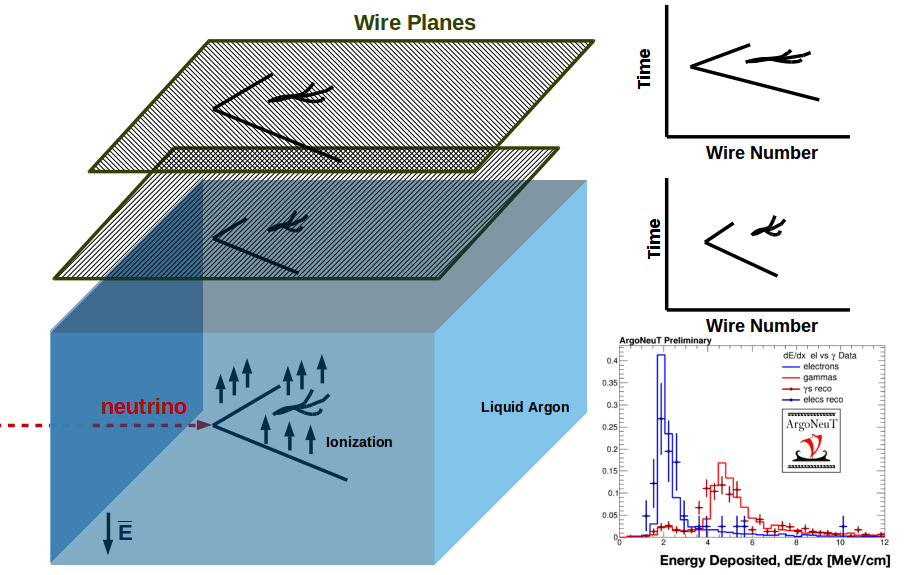
\includegraphics[width=0.55\textwidth]{images/lartpc.png}
\caption[]{Operating principals of LArTPC detectors.}
\label{fig:LArTPC}
\end{figure}

